\documentclass{article}
\usepackage[english]{babel}
\usepackage[utf8]{inputenc}
\usepackage{algorithm}
\usepackage[noend]{algpseudocode}
\usepackage{amsmath,amsfonts,amsthm}
\usepackage[letterpaper, margin=1.25in]{geometry}
\usepackage{apacite}
\usepackage{graphicx}

\title{Word2Vec: A Simplified Implementation in Java }
\author{Jacen Williams \\    
	    CS 4343 \\
	    University of Arkansas -- Fort Smith}
\date{\today}

\begin{document}
\maketitle

\begin{abstract}
	The Word2Vec project modifies the traditional Neural Network Language Model to efficiently and accurately produce word embeddings. These embedings can be used to compare words or as features for other Natural Language models. Producing these vectors, however, requires large datasets and a large amount of training time.
\end{abstract}

\section{Introduction}
Word embeddings are becoming an integral part of Natural Language Processing. They are used in a wide variety of techniques from Text Classification to Natural Language Generation. The Word2Vec project was created as an efficient means to create word embeddings on very large data sets\cite{efficient}. This technique produces unique, multi-dimensional vectors for each word in the dataset's vocabulary. These word vectors demonstrate multiple degrees of similarity\cite{efficient} such that they can be used to determine in what way words are similar. Further, basic algebraic operations can be performed on these vectors. For example: $vector("King") - vector("Man") + vector("Woman"$ is closest to the vector for the word $Queen$\cite{efficient}. This operation can be used to find pairs of words that are similar in the same way as another. In both of these models, the goal is not the output of the network, but rather the set of weights from the input to the hidden layer(or hidden to output layer for CBOW) for each word. The set of weights for a word is the vector embedding for that word.

\section{Background}

The original implementation by Mikolov et al. proposed two different models based on the Neural Language Model\cite{neural}. They called these models the CBOW(Continuous Bag of Words) and SkipGram models (\ref{fig:models}). While both models work similarly, their input and output are reversed. Both models are designed to use one-hot encoded vectors for input, with each position in the input vector referencing a unique word in the vocabulary. The CBOW model takes as input multiple vectors, each referencing a specific position in a window around the target word, and as output a vector containing the calculated probability of each word in the vocabulary being the target word. The Skip-gram model instead takes a single vector as input and outputs multiple vectors, each containing a probability distribution for a location in the window \cite{efficient}. Later research by Mikolov et al. focused on ways to improve this method, creating a method they dubbed "Negative Sampling" \cite{distributed}. This paper will focus on the Skip-gram model and Negative Sampling method.

\begin{figure}
	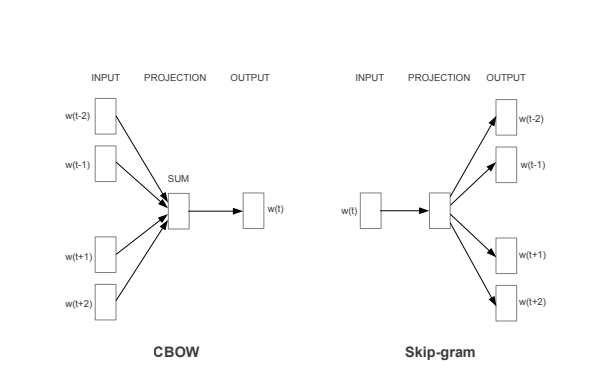
\includegraphics[width=\linewidth]{models.png}
	\caption{CBOW and SkipGram Models}
	\label{fig:models}
\end{figure}	

\section{Specification}

This implementation of Word2Vec uses a simplified version of the Skip-gram Model and Negative Sampling technique. Whereas the Skip-gram model outputs a probability distribution for each position in the context window, this implementation uses a "One-word context" \cite{parameter} approach. This method instead outputs a single probability distribution and trains the network for each word pair in the context window, with one word being the input, and the other the target. This method greatly simplifies the model. Negative Sampling is implemented to reduce the training time required for each input. The Skip-gram model uses a SoftMax output layer to normalize the output and then updates the weights of the Neural Network using back-propagation. Negative Sampling decreases the total training time by only training a small subset of output nodes. The number of nodes trained can vary but Mikolov et al. proposed that a range of 5-20 is best suited for small datasets while 2-5 is sufficient for large ones \cite{distributed}. The output nodes selected for training are selected randomly from a probability distribution, dubbed the "Unigram Distribution" \cite{distributed}. This distribution,  is created by adding each word into list $w$ times, with $w$ being a weight for each word calculated as $count(word)^x$ with x being a constant. In this implementation, x was chosen to be $3/4$ \cite{explained}. 

\section{Implementation}

The simplified implementation of Word2Vec is implemented in Java using Object Oriented Programming. The program consists of a main controller, capable of loading and testing data, and a neural network controller, which controls the neural model. The main controller has methods to load data, begin the network training sequence on loaded data, retrieve and print the vector for a single word or for all words in the vocabulary, and methods to test the data. The neural network controller has methods to instantiate a new network of a given size, perform the feed-forward and back-propagation functions of the network, and to return the derived vectors for a word. Training this model on a corpus of 250,000 words takes approximately 8 hours per epoch. This training time could be improved upon further by implementing other techniques mentioned by Mikalov et al. and modifying the simplified implementation to use multiple threads. 


\section{Evaluation}

Word vectors can be evaluated using the \emph{Semantic-Syntactic Word Relationship Test} \cite{efficient}. This test consists of two related word pairs which represent a specific semantic or syntactic relationship between the words  (\ref{fig:test}). 
\begin{figure}
	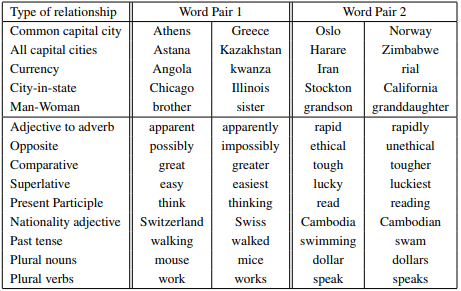
\includegraphics[width=\linewidth]{test.png}
	\caption{Semantic-Syntactic Word Relationship Test}
	\label{fig:test}
\end{figure}
These word pairs can be used to evaluate the accuracy of the model using $vector(pair1word1) - vector(pair1word2) + vector(pair2word1)$ comparing the output with the second word in the second pair. Two vectors can be compared using Cosine Distance, given as: 
$$
1 - \frac{\sum_{i=1}^{n} A_i B_i}{\sqrt{\sum_{i=1}^{n} A_{i}^{2}}\sqrt{\sum_{i=1}^{n} B_{i}^{2}}}
$$ with A and B being the word vectors. When performing the word comparison test, the word with the shortest cosine distance from the output vector is chosen as the most similar word. Training data was obtained from a subset the "One Billion Word Language Modeling Benchmark" dataset. Training data size was limited due to long training times and 250,000 words was the largest dataset used in this implementation. While Mikalov et al. were able to report accuracy as high as 65.6\%, the simplified model was not able to produce meaningful results with the current dataset size. Accuracy for the word comparison test approached 0\%. These results can likely be improved by training on larger datasets, however, in its current implementation, training a dataset large enough to produce meaningful results could take weeks or months.
\section{Conclusions}

While the Skip-gram and CBOW models have been shown to efficiently and accurately produce vector embeddings for words, the model must be trained on a very large dataset to  produce accurate results. Future work on this project will primarily be focused on methods to improve the training efficiency so that larger datasets may be used. 

\bibliographystyle{apacite}
\bibliography{References}




\end{document}